% Gerado automaticamente. No preambulo do documento use:
% \usepackage{pgfplots}
% \pgfplotsset{compat=1.18}
\definecolor{plotblue}{HTML}{2563EB}
\definecolor{plotorange}{HTML}{D97706}
\definecolor{plotgreen}{HTML}{059669}
\definecolor{plotpurple}{HTML}{7C3AED}
\definecolor{plotgray}{HTML}{374151}
\definecolor{plotred}{HTML}{DC2626}
\definecolor{plotteal}{HTML}{0F766E}
\definecolor{plotslate}{HTML}{64748B}

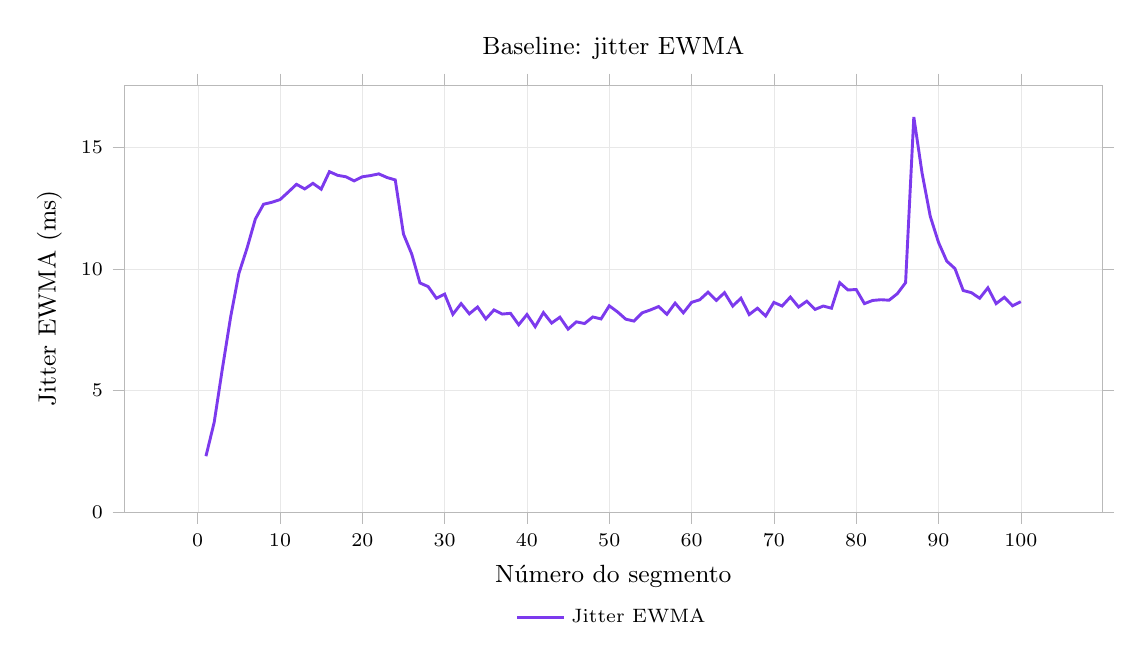
\begin{tikzpicture}
\begin{axis}[
    title={Baseline: jitter EWMA},
    xlabel={Número do segmento},
    ylabel={Jitter EWMA (ms)},
    width=14cm,
    height=7cm,
    grid=major,
    grid style={line width=.12pt, draw=gray!18},
    axis line style={draw=gray!55},
    tick style={draw=gray!55},
    tick align=outside,
    title style={font=\small},
    label style={font=\small},
    tick label style={font=\scriptsize},
    legend cell align={left},
    legend style={at={(0.5,-0.20)}, anchor=north, legend columns=2, draw=none, font=\scriptsize},
    ymin=0,
    ymax=17.5608
]
\addplot+[plotpurple, line width=1.05pt, mark=none] coordinates {
(1,2.3)
(2,3.69)
(3,5.91)
(4,8.03)
(5,9.82)
(6,10.87)
(7,12.06)
(8,12.67)
(9,12.75)
(10,12.86)
(11,13.17)
(12,13.49)
(13,13.3)
(14,13.53)
(15,13.29)
(16,14.01)
(17,13.86)
(18,13.8)
(19,13.63)
(20,13.8)
(21,13.85)
(22,13.92)
(23,13.77)
(24,13.67)
(25,11.44)
(26,10.62)
(27,9.43)
(28,9.28)
(29,8.8)
(30,8.97)
(31,8.14)
(32,8.58)
(33,8.16)
(34,8.44)
(35,7.95)
(36,8.32)
(37,8.15)
(38,8.18)
(39,7.71)
(40,8.13)
(41,7.63)
(42,8.21)
(43,7.78)
(44,8.02)
(45,7.53)
(46,7.83)
(47,7.76)
(48,8.03)
(49,7.95)
(50,8.49)
(51,8.24)
(52,7.94)
(53,7.86)
(54,8.2)
(55,8.32)
(56,8.46)
(57,8.14)
(58,8.6)
(59,8.2)
(60,8.63)
(61,8.74)
(62,9.05)
(63,8.71)
(64,9.03)
(65,8.48)
(66,8.8)
(67,8.13)
(68,8.39)
(69,8.07)
(70,8.63)
(71,8.48)
(72,8.85)
(73,8.44)
(74,8.68)
(75,8.34)
(76,8.48)
(77,8.39)
(78,9.44)
(79,9.14)
(80,9.16)
(81,8.58)
(82,8.71)
(83,8.74)
(84,8.72)
(85,8.99)
(86,9.44)
(87,16.26)
(88,13.96)
(89,12.17)
(90,11.1)
(91,10.33)
(92,10.02)
(93,9.12)
(94,9.03)
(95,8.8)
(96,9.23)
(97,8.58)
(98,8.84)
(99,8.49)
(100,8.66)
};
\addlegendentry{Jitter EWMA}
\end{axis}
\end{tikzpicture}
